\section{BC Policy Debugging Methodology}
\label{sec:methodology}

When a trained BC policy fails at evaluation time, the root cause can lie either in the policy itself (e.g., insufficient training, distributional shift) or in the observation pipeline (e.g., sensor noise, coordinate frame mismatches). Without a principled way to distinguish these failure modes, debugging degenerates into trial-and-error. We propose a four-step diagnostic methodology that has reliably isolated the root cause in our experiments.

\subsection{Step 1: Sanity Check --- Feed Training Observations to the Policy}
\label{sec:methodology:sanity}

The first and most informative diagnostic is to bypass the environment entirely and feed a recorded training observation directly to the policy. Concretely, we load one observation from the demonstration HDF5 file and query the policy:

\begin{lstlisting}[caption={Sanity check: feed a training observation to the policy.}]
import h5py
with h5py.File(train_hdf5, 'r') as f:
    train_obs = {k: f['data/demo_0/obs'][k][0]
                 for k in f['data/demo_0/obs'].keys()}
action = policy(train_obs)  # should be close to the demo action
\end{lstlisting}

The interpretation is binary:
\begin{itemize}[leftmargin=*,itemsep=2pt]
    \item If the policy outputs a reasonable action (close to the demonstration action recorded in the HDF5), the policy is \emph{not} the problem. The failure is in the observation pipeline at evaluation time.
    \item If the policy outputs a nonsensical action, the policy itself is broken. Likely causes: insufficient training, an incorrectly configured observation encoder, or a bug in the network forward pass.
\end{itemize}

In our case, the sanity check consistently passed: the policy produced reasonable actions on training observations. This ruled out a policy-side bug and focused our attention on the observation pipeline.

\subsection{Step 2: Observation Comparison --- Environment vs.\ Training}
\label{sec:methodology:obs_compare}

Having established that the policy is correct, we compare the evaluation environment's observation against the training observation, key by key:

\begin{lstlisting}[caption={Observation comparison: detect mismatches per key.}]
env_obs = env.get_observation()
for k in train_obs.keys():
    diff = np.abs(env_obs[k] - train_obs[k]).max()
    print(f"{k}: max_diff={diff:.4f}")
    if 'quat' in k and diff > 0.5:
        print(f"  WARNING: QUATERNION SIGN FLIP DETECTED")
\end{lstlisting}

The threshold $0.5$ for quaternion keys is chosen because a sign flip manifests as a maximum absolute difference approaching $2.0$ (e.g., $|0.71 - (-0.71)| = 1.42$), whereas legitimate numerical drift is typically below $0.01$. Any quaternion key with a maximum difference greater than $0.5$ is almost certainly sign-flipped.

For non-quaternion keys (e.g., \code{eef\_pos}, \code{gripper\_qpos}), a difference greater than $0.01$ indicates a coordinate-frame mismatch or a parameter change between data collection and evaluation.

\subsection{Step 3: Observation Isolation Test --- Replace One Key at a Time}
\label{sec:methodology:isolation}

When multiple observation keys differ, it is tempting to fix them all at once. This is a trap: fixing the wrong key first can mask the real problem. We instead perform an isolation test, starting from the (correct) training observation and replacing exactly one key at a time with the corresponding (suspicious) environment observation:

\begin{lstlisting}[caption={Isolation test: identify the single key responsible for failure.}]
for k in train_obs.keys():
    test_obs = {**train_obs, k: env_obs[k]}
    action = policy(test_obs)
    # if action degrades severely, key k is the culprit
\end{lstlisting}

The key whose replacement causes the largest action degradation is the root cause. In our experiments, this test unambiguously identified \code{robot0\_right\_eef\_quat} as the culprit, even when other keys also exhibited small numerical differences.

\subsection{Step 4: Transferability Test --- Same Object, Same Position}
\label{sec:methodology:transfer}

When a policy is trained on one task and needs to be deployed on a different task, the question is whether retraining is necessary. We propose a transferability test: if the target object and the end-effector initial pose are identical between two tasks, the policy can be transferred directly.

Concretely, we verify three conditions:
\begin{enumerate}[leftmargin=*,itemsep=2pt]
    \item The object's body position in the world frame is identical.
    \item The grasp site (left and right) positions are identical.
    \item The robot's base position is identical, hence the EEF initial pose is identical.
\end{enumerate}

When all three conditions hold, the policy trained on task A can be deployed on task B without retraining. In our benchmark, a single policy trained on level L3 transferred directly to levels L5, L7, and L9, saving multiple hours of training time per task.

\begin{figure}[htbp]
    \centering
    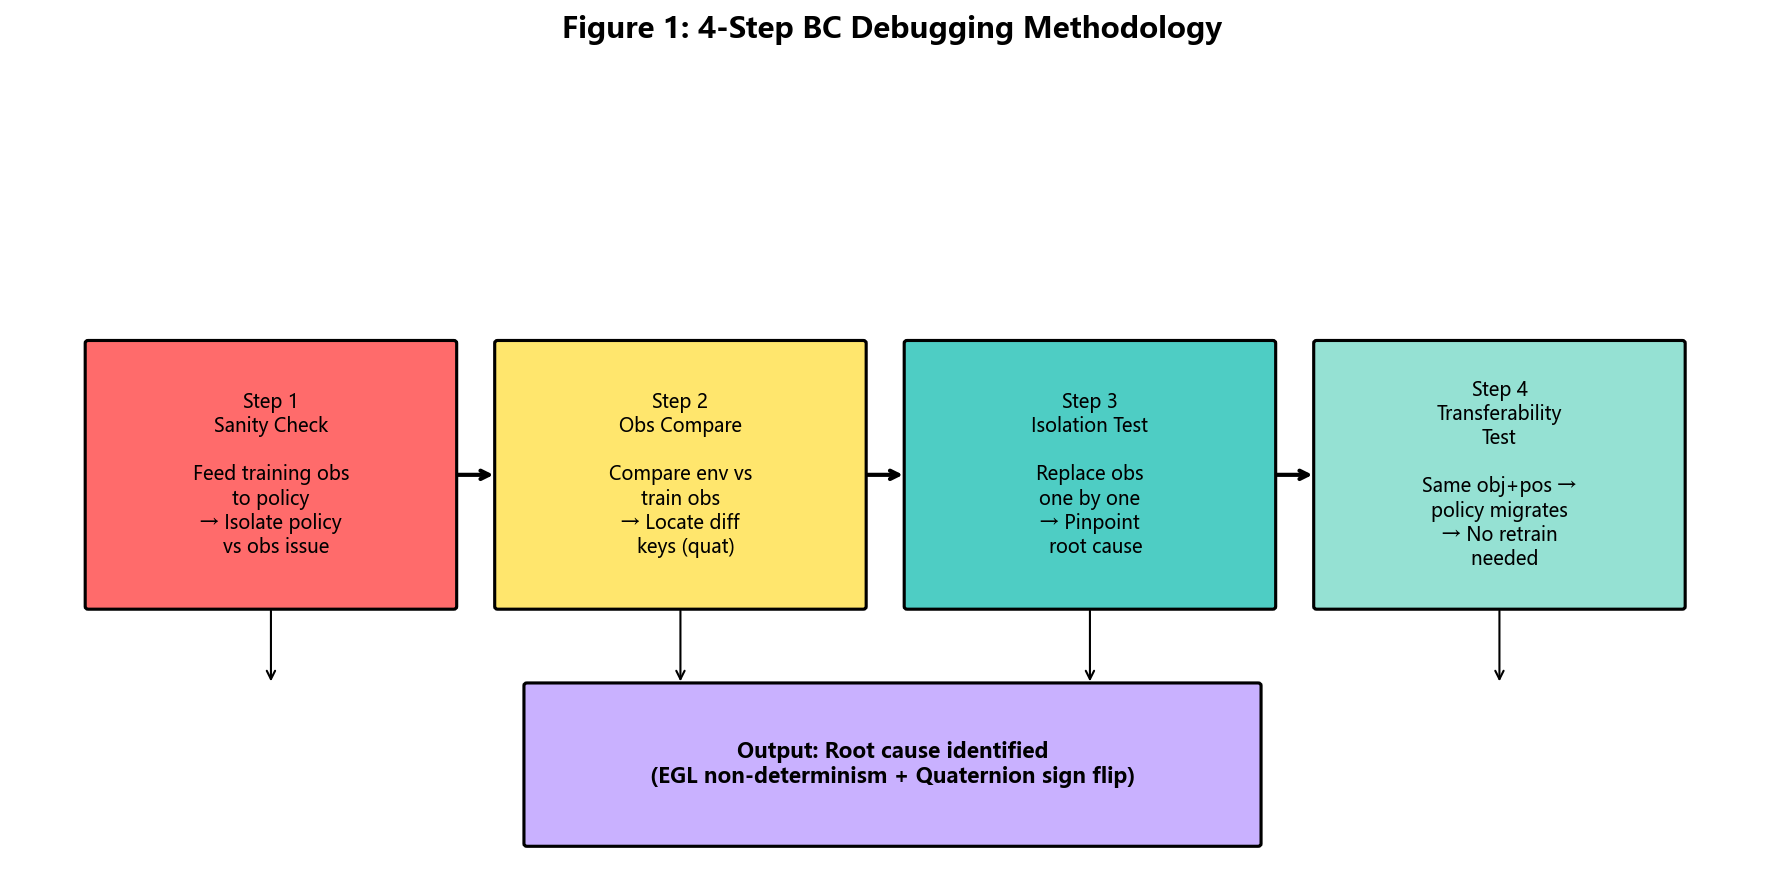
\includegraphics[width=0.95\textwidth]{figures/fig1_4step_diagnosis.png}
    \caption{The 4-Step BC Debugging Methodology decision tree. Each step narrows the search space from ``something is wrong'' to a specific observation key and a specific failure mode, culminating in the transferability test that determines whether retraining is necessary.}
    \label{fig:4step_diagnosis}
\end{figure}

\subsection{Summary}
\label{sec:methodology:summary}

The four steps form a decision tree, summarized in Table~\ref{tab:methodology}:

\begin{table}[h]
\centering
\caption{The 4-step BC debugging methodology.}
\label{tab:methodology}
\small
\begin{tabular}{p{0.15\textwidth} p{0.30\textwidth} p{0.45\textwidth}}
\toprule
\textbf{Step} & \textbf{Question} & \textbf{Action} \\
\midrule
1. Sanity check & Is the policy itself correct? & Feed training obs to policy. If action is reasonable, policy is fine. \\
2. Obs compare & Which keys differ? & Diff every observation key. Flag quat diffs $>0.5$. \\
3. Isolation & Which key is the root cause? & Replace one key at a time, measure action degradation. \\
4. Transferability & Can we avoid retraining? & Check if object + grasp site + base pos are identical. \\
\bottomrule
\end{tabular}
\end{table}

This methodology reliably narrows the search space from ``something is wrong'' to a specific observation key and a specific failure mode (e.g., quaternion sign flip), which can then be fixed with targeted interventions (Section~\ref{sec:quaternion}).
